\documentclass{article}
\usepackage{graphicx}
\usepackage{lipsum}
\usepackage{subcaption}
\usepackage{array}
\usepackage{multirow}
\usepackage{tabularx}
\begin{document}
\listoffigures
\bigbreak
\lipsum[1]

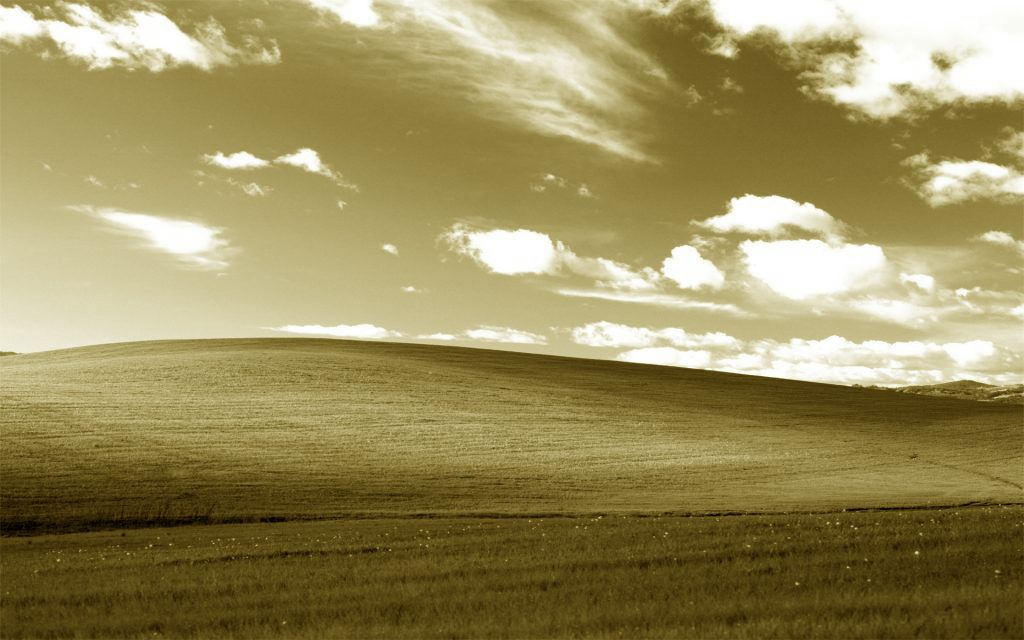
\includegraphics[width=5 cm, height=5 cm, keepaspectratio]{szepia.jpg}	
\lipsum[1]
\begin{figure}[ht]
\centering
\caption{Szines kep lol}
\label{fig:kepek}
	\begin{subfigure}[c]{5cm}
	\centering
	\caption{first}
	\smallbreak
	
\includegraphics[width=5 cm, height=5 cm, keepaspectratio]{szines.jpg}
	\end{subfigure}
\hspace{1em} % vízszintes helykihagyás
\bigbreak
\centering
\caption{Szepias kep lol}
	\begin{subfigure}[c]{5cm}
	\centering
	\caption{secondo}
	\smallbreak
	\framebox{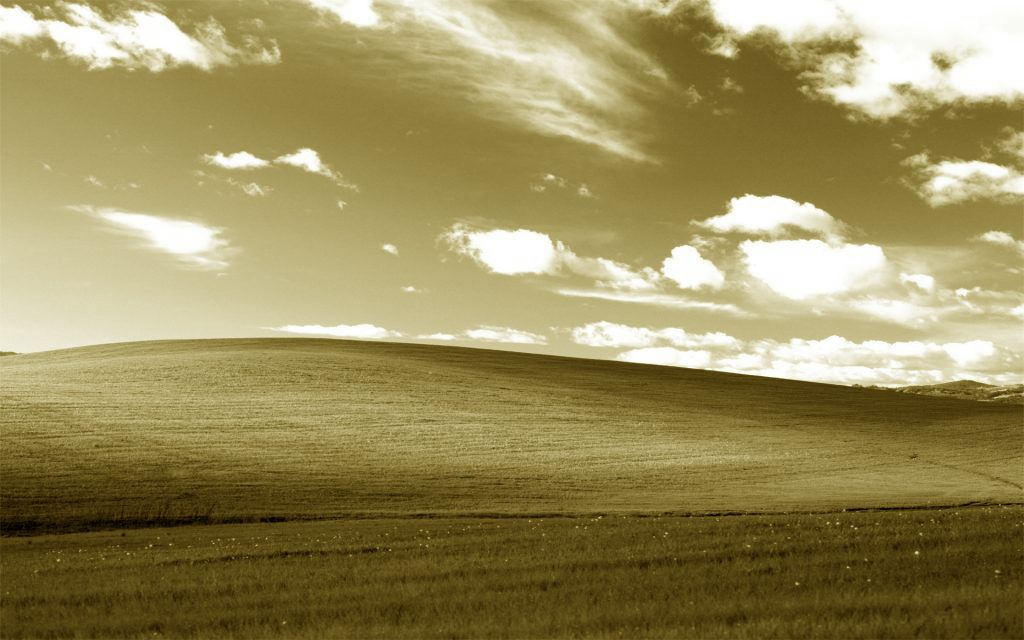
\includegraphics[width=5 cm, height=5 cm,angle=90]{szepia.jpg}}
	\end{subfigure}
\end{figure}
\bigbreak

\begin{center}


\begin{tabularx}{10 cm} {l|c|r}
\hline
  \hline
  cell1 dummy text & cell2 & cell3 \\ 
  \hline
  cell1 dummy text & cell5 & cell6 \\ 
  \hline
  cell7 & cell8 & cell9 \\ 
  \hline
   cell10 & cell11 & cell12 \\
  \hline
\end{tabularx}
\end{center}




\end{document}